\section{Seed Agent Model Discussion}

As a part of the creation of a our discrete-time model where numerous climate and regional factors contribute to the spread of dandelion plants, it is essential to conduct a sensitivity analysis to determine the most impactful factors on dandelion growth.

Beyond our sensitivity analysis, we also provide a brief discussion on the key strengths and weaknesses of our model, as well as a scope of how our model can be easily generalizable to virtually any plot of land.

\subsection{Model Hyperparameters}

Based on our model as described above, the following table consolidates all hyperparameters that can be changed per region calibration. Our sensitivity analysis as follows investigates the impacts of these hyperparameters on our model's predictions on the spread of dandelion plants and seeds.

\begin{table}[h]
\renewcommand{\arraystretch}{1.3}
%p{0.8\linewidth
    \begin{tabularx}{\textwidth}{p{0.2\textwidth}lp{0.4\textwidth}X}
    \toprule
    \textbf{Hyperparameter}  & \textbf{Symbol} & \textbf{Description} & \textbf{Default Value} \\ \midrule
    \raggedright Temperature & \(\tau(t)\)   & Temperature values over a year in a specific region in Fahrenheit. Dandelions grow optimally between 50 and \(77^\circ\) F (CITE). & Temperature from 2022 Clay, NY data (CITE!). \\
    \rowcolor{gray!15}
    \raggedright Light Levels & \(l(t)\)  & Hours of sunlight per day over a year. Dandelions grow optimally between 6 to 18 hours of sunshine per day (CITE)! & Average daily light in hours from 2022 Clay, NY data (CITE!).\\
    \raggedright Wind Levels & \(m(t)\) & Average mph of wind per day over a year which effects movement process. & Wind levels from 2022 in Clay, NY.  (CITE!!)\\
   \rowcolor{gray!15} \raggedright K Levels & \(k(t)\) & Average amount of Potassium in a regionally collected sample of soil in ppm over time. K levels accounts for soil moisture and richness (CITE!). & Potassium levels from a soil survey (CITE!).\\
      \raggedright N Levels & \(n(t)\) & Average amount of Nitrogen over time, a vital growth component of dandelions, in a regionally collected sample of soil in ppm. & Nitrogen levels from a soil survey (CITE!).\\
    \rowcolor{gray!15} \raggedright Seed Lifespan & \(\lambda_s(t)\) & Average time until death for dandelion seeds. & 4 days (CITE!) \\
    \raggedright Dandelion Lifespan & \(\lambda_d(t)\) & Average time until death or consumption for dandelion plants. & 15 days (CITE!) \\
     \rowcolor{gray!15} \raggedright Initial Seeds & \(S_0\) & Number of seeds dispersed by each dandelion in its puffball stage & 2000 seeds (CITE!)\\
    \bottomrule
    \end{tabularx}
\end{table}

\subsection{Sensitivity Analysis}

A common methodology for sensitivity analysis is to randomly sample various hyperparameter values and to analzye the output of our model. Therefore, to randomly sample different sets of hyperparameters for our model, we employed a Monte Carlo sampling simulation to randomly sample from \(\pm 10\%\) from initial conditions from our temperate climate region. 

Based on a Monte Carlo simulation sampling from a range of \(\pm 10\%\) from our model's default values of the hyperparameters, we modeled the effects of these changes on the growth of dandelion plant populations over time. These results are shown below.

\begin{figure}[h!]
\centering
    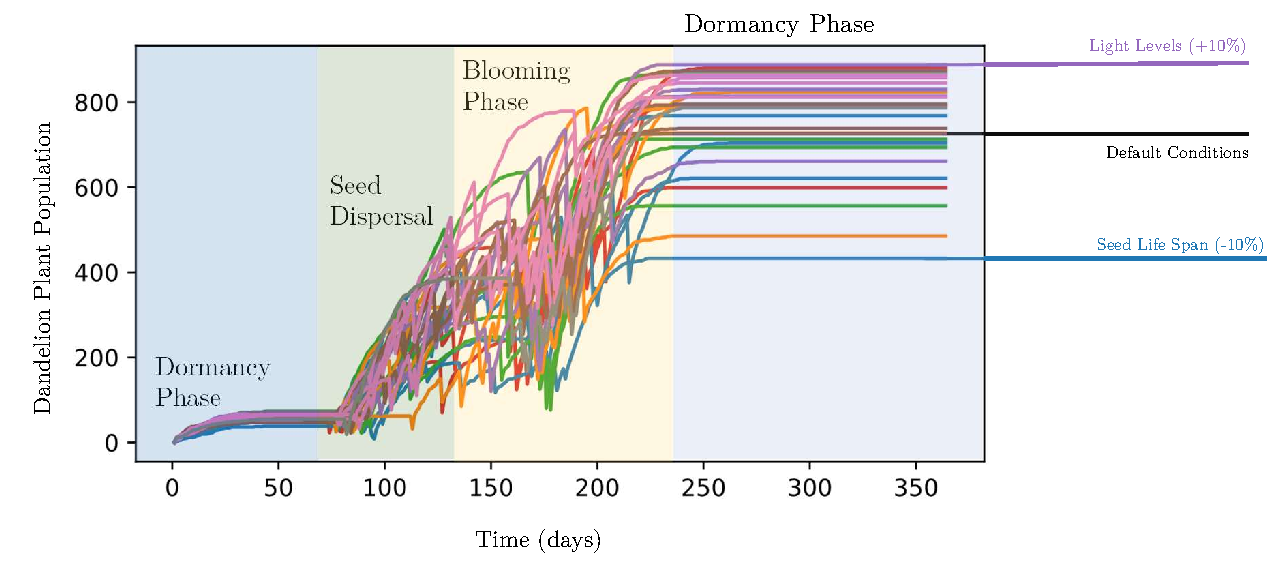
\includegraphics[scale=0.65]{figures/sensitivitypopulation.pdf}
    \captionsetup{width=0.9\textwidth}
    \caption{\textbf{Monte Carlo simulation sampling for hyperparameter sensitivity.}}
    \label{fig:sensitivitypopulation}
\end{figure}

From Figure~\ref{fig:sensitivitypopulation}, we demonstrate how despite changes in our model's hyperparameters, dandelion populations tend to follow the same three part process of dormancy, seed dispersal, and puffball blooming. At the end of the blooming phase, seeds are dispersed until the next blooming season reoccurs. Furthermore, dandelion plant populations generally asymptote towards a carrying capacity of the plot of land, which in our case, is dependent on a hyperparameter specifying the minimum distance between two dandelions necessary to survive.

To numerically analyze our results from Figure \ref{fig:sensitivitypopulation}, we analyzed the average Root-mean squared error (RMSE) between each factor's Monte Carlo simulation and our simulation with default conditions applied. The Root-mean-square error formula is commonly used in time-series analysis to determine the average deviation of a new time-series from a ground-truth series. Using the formula for RMSE where \(N\) is the number of entries compared,

\begin{equation}
    \text{RMSE} = \sqrt{\frac{1}{N}\sum\limits_{i=1}^{n} \left((x_{\text{new}_i} - x_{\text{ground truth}_i}\right)^2}
\end{equation}

we scaled each of these errors between \(0\) and \(1\) using min-max scaling and display our sensitivity analysis results in the radar chart below. Based on our analysis, light levels and seed lifespan have the greatest impacts on dandelion population growth (See Figure~\ref{fig:radarchart1}), which is consistent with findings from field observations (CITE!).

\begin{figure}[h!]
\centering
    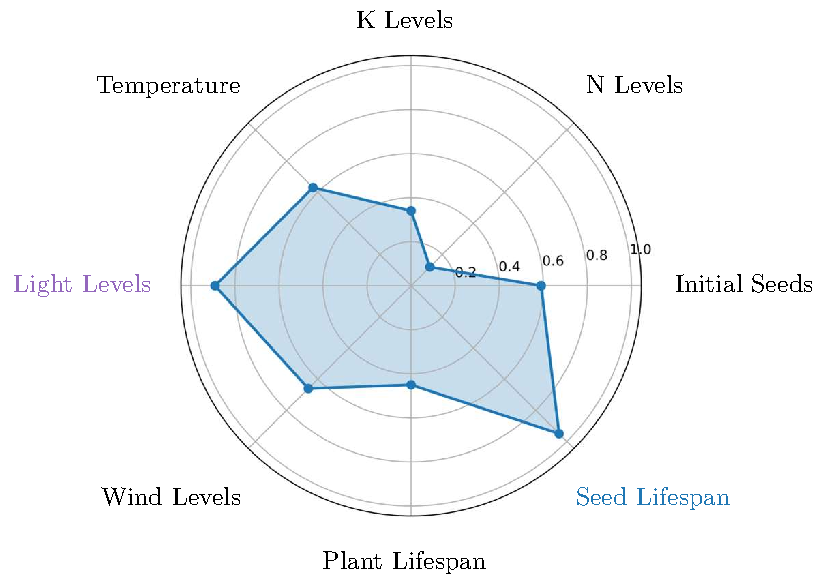
\includegraphics[scale=0.6]{figures/radarchart1.pdf}
    \captionsetup{width=0.9\textwidth}
    \caption{\textbf{Radar Chart of Model Hyperparameters.} The two most impactful factors of our model were the light levels and seed lifespan in the soil.} 
    \label{fig:radarchart1}
\end{figure}


\subsection{Strengths}

\begin{enumerate}
 \item Our main model’s strength is its ability to \textbf{powerfully generalize}.
    \begin{quote}
        For instance, through including numerous regional and climate hyperparameters into a single, robust framework, our model enables any investigator to thoroughly examine a plot of land for the growth of dandelions. Furthermore, all hyperparameters necessary can be easily obtained from soil samples and climate analysis.
    \end{quote}
    
\item We developed a \textit{theoretical probabilistic model} which \textbf{agrees with field observations}.
\begin{quote}
    Our unique combination of various stochastic processes provides an accurate and reliable framework for virtually any plot of land. Our use of probability analysis throughout the dandelion growth process can be adapted for other perenniel plants easily and make substantive conclusions for land use.
\end{quote}

\item A thorough Monte Carlo simulation and sensitivity analysis performed \textbf{helps dandelion growers} and watchers to best grow dandelions through our analysis of impact factors.
\begin{quote}
    Our analysis concluded that light levels and seed lifespans impact dandelion growth the most; therefore, dandelion harvesters must prioritize these factors above all others to ensure that dandelions can grow most optimally.
\end{quote}
\end{enumerate}

\subsection{Limitations}
\begin{enumerate}
\item Some special data for dandelions could not be found, and so we made \textbf{assumptions that seeds act as agents} and follow growth cycles based on some key climate parameters. 
\begin{quote}
    A more abundant data resource can guarantee a better accommodation for diverse climates in our models. For example occurrences of natural disasters, significant human interference, and specific consumer based behaviors would result in a more adept model. 
\end{quote}

\item Our model \textbf{derives climate and death rates from historical data}.
\begin{quote}
    Therefore, our model lacks predictive power for factors such as global warming and competition with other species. Between the fundamental trade-off of realism and model elegance, our model certainly tends towards realism with our use of stochastic processes.
\end{quote}
\end{enumerate}

